\documentclass[compress]{beamer}
\usetheme{Warsaw}
\usecolortheme{whale}

\usepackage{amsmath}
\usepackage{url}
\usepackage{graphicx}
\usepackage{pgf}
\usepackage{tikz}
\usetikzlibrary{arrows,automata}
\usepackage[latin1]{inputenc}
\usepackage{verbatim}

%Present bigger picture for intro.

%Concrete scenarios

%Clear about defining project: the OUR APPROACH slide!!



%In this particular project Web 2.0 not 1.0 like last time
%Why is this not applicable for threads...

%More data from the collected data...

%Maintain consistent terminologies. `Content-based features'
%HMM must explain more. Time gap.
%how it fits in.

\title{Predicting Web 2.0 Thread Updates\\Progress Update}
\author{Shawn Tan}

\setbeamertemplate{footline}{\insertframenumber/\inserttotalframenumber}
\AtBeginSection[]
{
\begin{frame}{Table of Contents}
\tableofcontents[currentsection]
\end{frame}
}

\date{}
\begin{document}
\maketitle
\section{Introduction}

\begin{frame}{Motivation}
	\begin{itemize}
		\item Many sites with thread-based discussion features
		\item Users post product reviews, feedback
	\end{itemize}
	Obtaining such up-to-date information may be vital to companies.
\end{frame}

\begin{frame}
\fontsize{6pt}{7.2}\selectfont
	\begin{table}\label{table:web20}
		{
		\begin{tabular}{|l|c|c|c|c|c|c|c|c|c|c|}
			\hline
				\input{web20}
			\hline
		\end{tabular}
		~\\
		}
		{
	\caption{Features of popular Web 2.0 sites}
		\begin{tabular}{l l}
			   T &= Twitter mentions\\
			FB L &= Facebook Likes \\
			FB S &= Facebook Shares\\
			G +1 &= Google +1 \\
			   L &= Likes (Local) \\
			  DL &= Dislikes (Local) \\
			   C &= Comments \\
			  PV &= Page Views \\
		 Follows &= Site-local feature for keeping track of user's activities
		\end{tabular}
	}
	\end{table}
\end{frame}


\begin{frame}
Ideally, an incremental crawler of such user-generated content should be able to maintain fresh content.

\end{frame}



\begin{frame}{Crawling forums: The Naive way}
	One way of keeping the database fresh, is to download pages at a frequent rate.

	However, forum sites are too large, with too many threads, incurring high bandwidth costs.

\textbf{Example:} \url{forums.hardwarezone.com.sg}
\begin{itemize}
	\item EDMW already has a total of 318615 threads\footnote{\url{http://forums.hardwarezone.com.sg/sitemap/f-16-p-1368.html}}.
\end{itemize}
\end{frame}
\begin{frame}
Using naive method:
	\begin{enumerate}
		\item incur excessive costs when downloading un-updated pages
		\item raise the possibility of the web master blocking the requester's IP address.
	\end{enumerate}

\end{frame}
\begin{frame}{Crawling forums: Estimating Future posts}
	Attempt to estimate future posts by learning from intervals between past posts.
% 	cite articles that use poisson distribution
\end{frame}
\begin{frame}{Extending current work}
	Use the content as well to attempt to make a better prediction.
	\begin{itemize}
		\item Technical forum discussions
		\item Flame wars (e.g. Vim vs. Emacs)
	\end{itemize}
	Threads in general have word signals that may hint at a different rate of updates.
	\begin{center}
		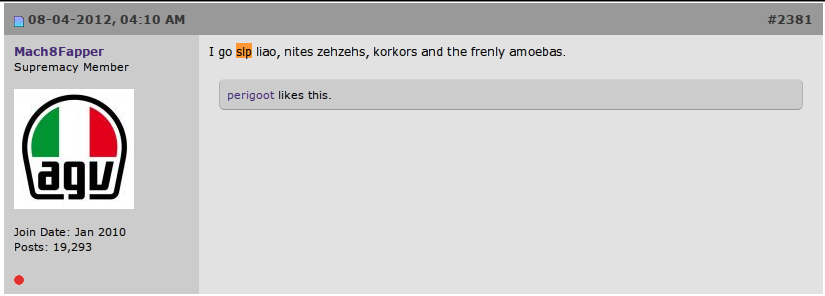
\includegraphics[scale=0.35]{nitez.png}
	\end{center}
%For example, a thread in a technical forum about a Linux distribution may start out as a question. Subsequent questions that attempt to either clarify or expand on the original question may then be posted, resulting in a quick flurry of messages. Eventually, a more technically savvy user of the forum may come up with a solution, and the thread may eventually slow down after a series of messages thanking the problem solver. Suppose 10 days later, someone with a slight variation of the same problem posts on the thread again. A crawler solely on the age of the thread to determine its download rate of the thread may not update itself with the thread.
\end{frame}



%TODO:Bring to beginning and shorten to 1 or 2 sentences after the problem statement.
%as rate increase, timeliness become more important
% talk about consequences of naive method


%Thus, we need a strategy of revisiting pages that will reduce the cost of downloading unchanged pages, while at the same time downloading them as soon as possible after it's update. 
%This year-long project proposes to use content-based features of a given thread to predict its next update time. We argue, that the content within the posts of the thread should be important in predicting the thread updates, and propose our approach to solving the problem.

\section{Related work}

\begin{frame}{Refresh policies for incremental crawlers}

Many works have used time difference to estimate page updates.
	\begin{enumerate}
		\item Coffman et. al. 1997 analysed the theoretical aspects.
		\item Cho and Garcia-Molina trace the change history of 720,000 web pages collected over 4 months.
		\begin{enumerate}		
			\item Showed empirically that the Poisson process model estimates the update processes well (Cho et. al. 1999)
			\item Proposed different revisiting or refresh policies (Cho et. al. 2003, Garcia-molina et. al. 2003)
		\end{enumerate}
		\item Also used in Tan et. al. 2007. %elaborate!!!!
	\end{enumerate}
\end{frame}

\begin{frame}{Problems with Poisson}
	The Poisson distribution is memoryless, and in experimental results due to Brewington and Cybenko 2000, the behaviour of site updates are not. 
\end{frame}

\begin{frame}{Using Site-level Knowledge}
Yang et. al. 2009, attempted to resolve this by
	\begin{enumerate}
		\item Using the list structure of forum sites to infer a sitemap.
		\item Use a linear-regression model to predict when the next update to the thread will arrive. %elaborate!!!
		\item Linear model used together with the sitemap information to prioritise the request queue in the crawler.
		\item Has the ability to make use of index information to infer changes in threads. Other types of comment systems do not have such indices.
	\end{enumerate}
\end{frame}
\begin{frame}{Summary}
	\begin{itemize}
		\item Previous work dealt with Web 1.0 sites.
		\item Did not take into account the content in the posts.
		\item Evidence to show that using time, while makes reasonable prediction, does not fully model the behaviour of threads.
	\end{itemize}
\end{frame}

%Online forums and bulletins have a logical, hierarchical structure in their layout, which typically alerts the user to thread updates by putting threads with new replies at the very top of the thread index. Yang's work exploits this as well as their linear model to achieve a predicton of when to retrieve the pages.
%However, this is not so for comments found on blog sites or discussion threads in an e-commerce site about a certain product and the lack of these pieces of information may result in a poorer estimate, or no estimate at all.

%Our perspective is that the available content on the thread at the time of the retrieval should also be factored into the model used to predict the page updates. Next, we look at some of the related work pertaining to thread content.

%\begin{frame}{Should include?}
%Wang et. al \cite{Wang2011} did work in finding out linkages between forum posts using lexical chaining. They proposed a method to link posts using the tokens in the posts called $Chainer_{SV}$. While they do analyse the content of the individual posts, the paper does not make any prediction with regards to newer posts. The methods used to produce a numeric similarities between posts may be used as a feature to describe a thread in its current state, but incorporating this into our model is non-trivial.
%\end{frame}


%Kleinberg used Hidden Markov Models to predict ``bursts" in message arrival times \cite{Kleinberg2003}. In his running example, he used email messages, and used time between messages to estimate the states that produced the sequence. While the model may be able to predict what the state is for the next time interval, it does so using the history of message arrival times, and does not take into account the content within the messages themselves.


%One also cannot ignore the fact that social factors play a role when users interact in an online discussion. Granovetter's threshold model for social behaviour may also be useful in describing how the users behave as a whole.
\section{Preliminary Work}
\begin{frame}{Extracting Data}
	Collected data from \url{forums.hardwarezone.com.sg}, \url{avsforum.com} as our data set.
	\begin{itemize}
		\item User
		\item Timestamp
		\item Message body
	\end{itemize}
\end{frame}


\begin{frame}{Preliminary experiments}
We picked a few threads (more than 3 days):
\begin{enumerate}
	\item Computed time difference between posts $\Delta t$
		\[
			\hdots~~p_i\underbrace{~~~~~~~~}_{\Delta t_i} p_{i+1}~~\hdots
		\]
	\item Sort posts by time difference
	\item Use median of $\Delta t$ as splitting point
	\item Train a Naive Bayes classifier using bag-of-words model to classify posts into 2 categories:
	\begin{itemize}
		\item $\Delta t > 6$
		\item $\Delta t \leq 6$
	\end{itemize}
\end{enumerate}
\end{frame}

\begin{frame}{Results}

\begin{table}
	\label{table:naivebayesresults}
	\makebox[\textwidth][c]{
		\begin{tabular}{|l|c|c|c|}
			\hline
			Class				& Precision	& Recall	&	$F_1$ \\
			\hline
			$\Delta t \leq 6$	& 0.657 & 0.816 & 0.728 \\
			$\Delta t >    6$	& 0.682 & 0.483 & 0.565 \\
			Overall				& 0.670 & 0.650 & 0.647 \\
			\hline
		\end{tabular}
	}
	\caption{Naive Bayes classification results}
\end{table}
\begin{enumerate}
	\item 10-fold cross validation for results
	\item Low recall value for $\Delta t > 6$. May be due to overlapping terms in vocabulary resulting in $\Delta t> 6$ posts being wrongly classified.
\end{enumerate}
Suggests that there is a relationship between content and update rates.
\end{frame}

%\begin{frame}{User posting frequency}
%\begin{figure}\label{sleepcycle}
%\makebox[\textwidth][c]{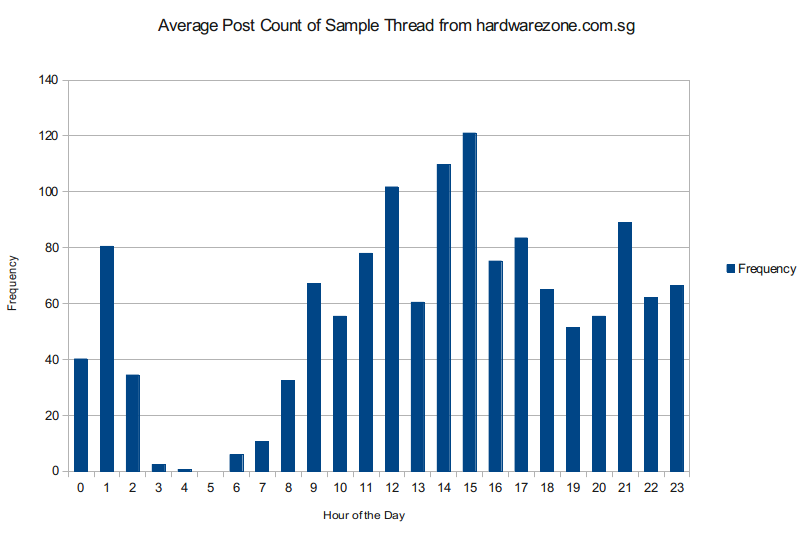
\includegraphics[scale=0.35]{threadfreq.png}}
%\end{figure}
%Thread update rates also dependent on users' sleep cycle
%\end{frame}
%The low recall for $\Delta t > 6$ may be due to a high number of overlapping terms in its vocabulary, causing a high number of false negatives. However, the results do suggest that there is some relationship between the content and $\Delta t$s that are less than or equal to 6 minutes. 


%We intend to implement the algorithm used in Yang et. al. \cite{Yang2009}, as a baseline to evaluate our system. However, since the algorithm uses the overall sitemap as additional information, only the linear regression model used to predict future incoming posts will be used. We will also use an SVM, trained using discretised time intervals and the extracted feature vectors.

%Compare with graph in paper... timeliness vs bandwith..
\begin{frame}{Yang et. al. 2009 Linear model}
	We wanted to evaluate how well the linear model performs without the sitemap information:
	\begin{enumerate}
		\item Implemented linear model from Yang et. al. 2009
			\begin{enumerate}
				\item Used time based features (e.g. Average $\Delta t$, Day of week, Hour of day)
			\end{enumerate}
		\item Trained against data from \url{http://avsforum.com}
		\item Compared against model that uses the average previous 5 $\Delta t$ values.
	\end{enumerate}
\end{frame}

\begin{frame}{Modifications to model}
	\begin{enumerate}
		\item Used baseline method (average of previous 5) if linear model returns a negative value.
		\item Revisits at the same predicted time interval when there's no change to the thread.
	\end{enumerate}
\end{frame}
\begin{frame}{Evaluation metric}
To evaluate \emph{timeliness} we use the metric employed in Yang et. al. 2009
\[
	T = \frac{1}{N} \sum^{N}_{i=1}\Delta t_i
\]
\end{frame}
\begin{frame}
\[
	\uparrow~~p_1,\underbrace{~~p_2,\underbrace{~~p_3,\underbrace{~~}_{\Delta t_3}}_{\Delta t_2}}_{\Delta t_1}\uparrow
\]
\textit{Problem:} A crawler that hits the site repeatedly performs well according to this metric.
\begin{enumerate}
	\item Limited by daily bandwidth (No. of pages)
	\item If bandwidth used up, downloads the next day, which contributes to overall $T$
\end{enumerate}
\end{frame}


\begin{frame}{Results}
	The linear model performed worse than the 5-average model. Values rounded up to nearest minute:
	\begin{itemize}
		\item Average Baseline Timeliness: 2490 minutes
		\item Average LM Timeliness: 3469 minutes
		\item Average paired difference (LM $-$ Baseline): 980 minutes
	\end{itemize}
	Model working as part of the larger overal framework as seen in Yang et. al. 2009 may give better results than just the linear model by itself.
\end{frame}
\section{Work Plan}


\begin{frame}{Week 3 - Week 4}
	Implementation of baselines
	\begin{itemize}
		\item Yang et. al. 2009 linear regression
		\item Discretised values using classification
			\begin{itemize}
				\item Try to predict classes or bins of $\Delta t$ values
			\end{itemize}
	\end{itemize}
\end{frame}

\begin{frame}{Week 5 - Week 9}
	Explore other possibilities for prediction.\\
	Some considerations:
	\begin{enumerate}
		\item Adaptive model
		\item Efficiency
		\item Predicting Responses to Microblog Posts (Artzi et. al. 2012)
			\begin{itemize}
				\item Use social data
			\end{itemize}
	\end{enumerate}
\end{frame}

%\begin{frame}{Thread States}
%	\begin{itemize}
%		\item Threads governed by probabilistic state machine
%		\item Each state has an associated update rate, and set of observations (content-based)
%	\end{itemize}
%\end{frame}
%\begin{frame}{Hidden Markov Model}
%\begin{columns}[c]
%\column{1.5in}
%\scalebox{0.5}{
%	\begin{tikzpicture}[->,>=stealth',shorten >=1pt,auto,node distance=3.5cm,semithick]
%	  \tikzstyle{every state}=[fill=blue,draw=none,text=white]
%
%	  \node[initial,state] (q0)                    {$q_0$};
%	  \node[state]         (IN) [below of=q0] {$q_I$};
%	  \node[state]         (AD) [left of=IN] {$q_{AD}$};
%	  \node[state]         (AN) [right of=IN] {$q_{AN}$};
%	  \path (q0) edge              node {} (AD)
%				 edge 			   node {} (AN)
%				 edge 			   node {} (IN)
%			(AD) edge [loop above] node {}(AD)
%				 edge [bend left]  node {}(AN)
%				 edge [bend left]  node {}(IN)
%			(AN) edge [bend left]  node {}(AD)
%				 edge [loop above] node {}(AN)
%				 edge [bend left]  node {}(IN)
%			(IN) edge [bend left]  node {}(AD)
%				 edge [bend left]  node {}(AN)
%				 edge [loop below] node {}(IN);
%	\end{tikzpicture}
%}
%\column{3in}
%\begin{description}
%	\item[$q_0$] Initial thread state when only 1 post.
%	\item[$q_I$] Idle thread state.
%	\item[$q_{AD}$] Active thread during `day'.
%	\item[$q_{AN}$] Active thread during `night'.
%\end{description}
%\end{columns}
%\end{frame}
%
%\begin{frame}{State observations}
%In the case of our thread content, possible content-based observations include:
%\begin{itemize}
%	\item Average length of a post
%	\item Word frequencies
%	\item Time between posts
%\end{itemize}
%%Since new posts are more likely to be influenced by more recent posts, a form of weighted importance should be introduced, giving the later posts greater influence on the prediction.
%\end{frame}

\begin{frame}{Week 10 (Optimistic) - Week 13}
	Evaluation of the method if completed.
\end{frame}
\end{document}
